\documentclass[a4paper]{article}

\usepackage[english]{babel}
\usepackage[utf8]{inputenc}
\usepackage[T1]{fontenc}       %makes text copy-and-pastable
\usepackage{wrapfig}           %for figures
\usepackage{graphicx}          %for images
\usepackage{booktabs}          % good tables package
\usepackage{array}             %for spacing tables
\usepackage{multirow}          %for multirow tables
\usepackage{caption}           %for the captionof command
\usepackage{amsmath}           %for any moderately complex math
\usepackage{placeins}          %allows us to use \FloatBarrier
\usepackage{caption}           %to use minipage for inserting figures
\usepackage{float}             %for H figure and table placements Here.
\usepackage{comment}          %for bulk comments
\usepackage[colorinlistoftodos, disable]{todonotes}%to do notes
\usepackage[parfill]{parskip}  %To use blank lines instead of indentation to separate paragraphs
\usepackage{ifthen}            %ifthenelse command
\usepackage[margin=3cm]{geometry} %Change margin size
\usepackage{titling}           %for spacing the title
\usepackage{blindtext}         %for spacing the title
    \setlength{\droptitle}{-4em}     % For spacing the title
    \addtolength{\droptitle}{-4pt}   % For spacing the title
%\usepackage[super]{nth}        %write 1st,2nd,3rd with \nth{1},\nth{2}, \nth{3}
%\usepackage{ifdraft}
\usepackage{units}
\usepackage{subcaption} % for subfigures
\captionsetup{width=0.8\textwidth}


\usepackage{tikz}
\usepackage{calc}
% \usepackage{pgfgantt}             %For gantt charts
\usepackage{pgffor}
\usepackage[american]{circuitikz}
\usepackage{ifthen}
\usepackage{pgfplots}
\pgfplotsset{compat=1.13}
\usetikzlibrary{decorations.pathreplacing}

\usepackage{varioref}

\listfiles

\usepackage[hidelinks,%clickable cross references and URLs
            pdftex,%pdf meta data
            pdfauthor={Matthew Davis},%pdf meta data
            pdftitle={ELEC4614 2013 Solutions},%pdf meta data
            %pdfsubject={\@title},%pdf meta data
            pdfkeywords={UNSW, ELSOC, ELEC4614, Power, Electronics, Past, Paper, Exam, Solutions}]{hyperref}

\usepackage[nameinlink, capitalise, noabbrev]{cleveref}

\title{ELEC4614 2013 S1 Exam Solutions}
\author{Matthew Davis \\ \href{mailto:vicepresident@elsoc.net}{vicepresident@elsoc.net}}

\renewcommand\thesection{Question \arabic{section}}
\renewcommand\thesubsection{(\alph{subsection})}
\renewcommand\thesubsubsection{\roman{subsubsection})}

\usepackage{tocloft}
\usepackage{chngcntr}
\setlength{\cftsecnumwidth}{6em}
%\setlength{\cftsubsecnumwidth}{3.25em}
\setlength{\cftsubsubsecnumwidth}{4em}


\pgfplotsset{
    standard/.style={
        axis x line=middle,
        axis y line=left,
        xlabel style={align=right}, 
        ticklabel style={fill=white},
        set layers=tick labels on top% use layers and choose the new layer set
    },
    layers/tick labels on top/.define layer set=% define the new layer set based on the standard one
        {axis background,axis grid,axis ticks,axis lines,main,%
          axis tick labels,% <- tick labels before main
          axis descriptions,axis foreground}
        {/pgfplots/layers/standard}
}



\begin{document}

\maketitle

\begin{abstract}
    These are the unofficial solutions to the 2013 Semester 1 Power Electronics exam.
    There are two different 2013 exams. 
    These solutions are for the one where question 1a has no inductor. The questions are available on the Library website.
    The other exam is the supplementary exam, on Moodle, with `2012' in the filename.
    This is just the first draft. I don't guarantee than the solutions here are correct. If you spot a mistake, please let me know. I've put orange boxes throughout to indicate where I'm unsure.
    More solutions, papers and notes can be found at \href{www.elsoc.net}{elsoc.net}.
    Please note that for this particular exam, you only needed to solve 4 out of 6 possible questions.
\end{abstract}

%\listoftodos

\tableofcontents

\section{Half-Wave Rectifiers}


% 1-wt
% 2 - alpha
% 3 - beta
\pgfmathdeclarefunction{truncSin}{3}{%
  \pgfmathparse{%
    (and(1,mod(#1,360)<=#3)*
    (and(1,mod(#1,360)>=#2)*
    (sin(#1))
    }%
}


% 1 - wt
% 2 - w
% 3 - R
% 4 - L
% 5 - phi
\pgfmathdeclarefunction{IL}{5}{%
  \pgfmathparse{%
     (
        sin((#1)-(#5))
        +sin(#5)*exp(-1*(#3)*((mod(#1,360)*0.02/360))/(#2*#4))
      )
    )
    }%
}
\xdef\uncontrolledRectifierGraphWidth{20}
\subsection{}\label{sec:1a}

Assuming that the voltage source has amplitude $V_s$, not $\sqrt{2}V_s$.

\begin{center}


% \begin{figure}[htbp]
%     \centering
%     \begin{subfigure}[b]{\linewidth}
%       \centering
       
\begin{tikzpicture}%[node distance = 2 cm, scale=1]


\begin{axis}[standard,
             domain=0:400, 
             xtick={180,360}, 
             xticklabels={$\pi$,$2\pi$},
             ytick={-1,1},
             yticklabels={$-V_s$,$V_s$},
             xlabel={$\omega{}t$},
             width=0.8\textwidth,
             xlabel style={align=right}, 
             height=6cm,
             %width=\uncontrolledRectifierGraphWidth,
             ymax=1.2,
             ymin=-1.2,
             ] 
    \addplot[dashed, red, domain=180:360] {sin(x)}; 
    \addplot[blue, samples=360] {truncSin(x,0,180)};  
    \legend{$v_S$, $v_L$}
\end{axis}


\end{tikzpicture}
    %   \caption{Supply voltage ($v_S$) and load voltage ($v_L$)}
    %   \label{1a fig:uncontrolled voltage graph}
    % \end{subfigure}
    \vspace{2cm} \\
    % \begin{subfigure}[b]{\linewidth}
    %   \centering
       
\begin{tikzpicture}%[node distance = 2 cm, scale=1]


\begin{axis}[standard,
             domain=0:400, 
             xtick={180,360}, 
             xticklabels={$\pi$,$2\pi$},
             ytick={0,1},
             yticklabels={{\color{white}$-V_s$},$\frac{V_s}{R}$},
             xlabel={$\omega{}t$},
             width=0.8\textwidth,
             xlabel style={align=right}, 
             height=6cm,
             %width=\uncontrolledRectifierGraphWidth,
             ymax=1.2,
             %ymin=0,
             ] 
    \addplot[green, samples=360] {truncSin(x,0,180)}; 
    \legend{$i_L$}
\end{axis}


\end{tikzpicture}
%       \caption{Load current ($i_L$)}
%       \label{1a fig:uncontrolled current graph}
%     \end{subfigure}
%     \caption{Current and voltage waveforms for Q1a}
%     \label{1a fig:uncontrolled rectifier graphs}
% \end{figure}
\end{center}

\begin{align*}
V_{AV} & = \frac{1}{2\pi} \int_0^{2\pi} V_L(\omega{}t) d \omega t \\
       & = \frac{1}{2\pi} \int_0^{\pi} V_s\sin(\omega{}t) d \omega t \\
       & = \frac{V_s}{2\pi} \left[ -\cos(\omega{}t) d \right]_0^{\pi} \\   
       & = \frac{V_s}{2\pi} \left[ --1 --1 \right] \\   
       & = \frac{V_s}{\pi} \\
\intertext{\todo[inline]{Hmm. Is that right?}}
I_{AV} & = \frac{V_{AV}}{R} \\
       & = \frac{V_s}{R\pi}
\end{align*}


\subsection{}

\begin{center}
% \begin{figure}[htbp]
    \xdef\myBeta{225.787377}
    % \centering
    % \begin{subfigure}[b]{\linewidth}
    %   \centering
       
\begin{tikzpicture}%[node distance = 2 cm, scale=1]

\begin{axis}[standard,
             domain=0:400, 
             xtick={180,\myBeta,360}, 
             xticklabels={$\pi$,$\beta$,$2\pi$},
             ytick={-1,1},
             yticklabels={$-V_s$,$V_s$},
             xlabel={$\omega{}t$},
             xlabel style={align=right}, 
             width=0.8\textwidth,
             height=6cm,
             %width=\uncontrolledRectifierGraphWidth,
             ymax=1.2,
             ymin=-1.2,
             ] 
    \addplot[dashed, red, domain=\myBeta:360] {sin(x)}; 
    \addplot[blue, samples=400] {truncSin(x,0,\myBeta)};  
    \legend{$v_S$, $v_L$}
\end{axis}


\end{tikzpicture}
    %   \caption{Supply voltage ($v_S$) and load voltage ($v_L$)}
    %   \label{fig:1b uncontrolled voltage graph}
    % \end{subfigure}
    \vspace{2cm} \\
    % \begin{subfigure}[b]{\linewidth}
    %   \centering
       
\begin{tikzpicture}%[node distance = 2 cm, scale=1]



\xdef\myOmega{2*3.1415*50}
\xdef\resistance{100}
\xdef\inductance{1}
\pgfmathparse{atan(\myOmega * \inductance / \resistance)}
\xdef\myPhi{\pgfmathresult}


\begin{axis}[domain=0:400, 
             axis x line=middle, 
             axis y line=left, 
             xtick={180,\myBeta,360}, 
             xticklabels={$\pi$,$\beta$,$2\pi$},
             ytick={0}, 
             yticklabels={\color{white}$-V_s$},
             x axis line style={->},
             xlabel={$\omega{}t$},
             xlabel style={align=right}, 
             ymax=1.5,
             y axis line style={->},
             width=0.8\textwidth,
             height=6cm,
             %width=\uncontrolledRectifierGraphWidth,
             ] 
    % 1 - wt
    % 2 - w
    % 3 - R
    % 4 - L
    % 5 - phi
    % \addplot[green, samples=360]
    % {(and(1,mod(x,360)<\myBeta)*IL(x,\myOmega,\resistance,\inductance,\myPhi)};  
    \input{1/figures/b/timeCoords}
    \legend{$i_L$}
    
\end{axis}

\end{tikzpicture}
%       \caption{Load current ($i_L$)}
%       \label{fig:1b uncontrolled current graph}
%     \end{subfigure}
%     \caption{Current and voltage waveforms for Q1b}
%     \label{fig:1b uncontrolled rectifier graphs}
% \end{figure}
\end{center}

\begin{align*}
V_L & = \frac{1}{2\pi} \int_0^\beta V_s \sin(\omega t) d \omega t \\
    & = \frac{V_s}{2\pi} \left[ -\cos(\omega t) \right]_0^\beta \\
    & = \frac{V_s}{2\pi} \left[ 1- \cos(\beta) \right]_0^\beta \\
\end{align*}


\subsection{}

\begin{center}
% \begin{figure}[htbp]
%     \centering
%     \begin{subfigure}[b]{\linewidth}
%       \centering
       
\begin{tikzpicture}%[node distance = 2 cm, scale=1]

\begin{axis}[domain=0:400, 
             axis x line=middle, 
             axis y line=left, 
             xtick={180,360}, 
             xticklabels={$\pi$,$2\pi$},
             ytick={-1,1},
             yticklabels={$-V_s$,$V_s$},
             x axis line style={->},
             xlabel={$\omega{}t$},
             xlabel style={align=right}, 
             y axis line style={->},
             width=0.8\textwidth,
             height=6cm,
             %width=\uncontrolledRectifierGraphWidth,
             ymax=1.2,
             ymin=-1.2,
             ] 
    \addplot[dashed, red, domain=180:360] {sin(x)}; 
    \addplot[blue, samples=400] {truncSin(x,0,180)};  
    \legend{$v_S$, $v_L$}
\end{axis}


\end{tikzpicture}
    %   \caption{Supply voltage ($v_S$) and load voltage ($v_L$)}
    %   \label{1c fig:uncontrolled voltage graph}
    % \end{subfigure}
    \vspace{2cm} \\
    % \begin{subfigure}[b]{\linewidth}
    %   \centering
       
\begin{tikzpicture}%[node distance = 2 cm, scale=1]


\begin{axis}[domain=0:400, 
             axis x line=middle, 
             axis y line=left, 
             xtick={180,360}, 
             xticklabels={$\pi$,$2\pi$},
             ytick={},
             %yticklabels={$-V_s$,$V_s$},
             x axis line style={->},
             xlabel={$\omega{}t$},
             xlabel style={align=right}, 
             y axis line style={->},
             width=0.8\textwidth,
             height=6cm,
             %width=\uncontrolledRectifierGraphWidth,
             ymax=1.2,
             ymin=-1.2,
             ] 
    \addplot[green, samples=360] {
    (and(1,mod(x,360)<180)* (0.5-0.4*cos(x)))
    +(and(1,mod(x,360)>=180)* (0.9 * exp(-(x-180)*0.01155)))
    };  
    \addplot[dotted, domain=360:400] {
    +(0.9 * exp(-(x-180)*0.01155))
    };  
    
    \legend{$i_L$}
\end{axis}

\end{tikzpicture}
%       \caption{Load current ($i_L$)}
%       \label{1c fig:uncontrolled current graph}
%     \end{subfigure}
%     \caption{Current and voltage waveforms for Q1c}
%     \label{1c fig:uncontrolled rectifier graphs}
% \end{figure}
\end{center}

The load current is sinusoidal with an offset in the first half of each period.
In the second half it's decaying exponentially towards zero, with time constant $\frac{L}{R}$.


The average voltage is now the same as for part a.
$$
V_L = \frac{V_s}{R\pi}
$$
\subsection{}

\begin{align*}
Z & = \sqrt{R^2 + (\omega L)^2} \\
  & = \sqrt{10^2 + (2\pi \times 50 \times  0.1)^2} \\
  & = \unit[32.969]{\omega} \\
\Phi & = \tan^{-1}\left(\frac{\omega L}{R}\right) \\
     & = \tan^{-1}\left(\frac{2\pi \times 50 \times 0.1}{10}\right) \\
     & = 72.34^\circ
\end{align*}

I'm going to use roughly a binary search.
$\beta$ could lie from $180^\circ$ to $360^\circ$. So let's start in the middle.

\begin{align*}
i(270^\circ) & = \frac{230\sqrt{2}}{32.969} \sin(270^\circ) - 72.34^\circ) = -2.992 \\
\intertext{Negative, so let's go smaller.}
i(225^\circ) & = \frac{230\sqrt{2}}{32.969} \sin(225^\circ) - 72.34^\circ) = +4.5311 \\
\intertext{Positive, so let's go larger.}
i(255^\circ) & = \frac{230\sqrt{2}}{32.969} \sin(255^\circ) - 72.34^\circ) = -0.4 \\
i(250^\circ) & = \frac{230\sqrt{2}}{32.969} \sin(250^\circ) - 72.34^\circ) = +0.4 \\
i(252.5^\circ) & = \frac{230\sqrt{2}}{32.969} \sin(252.5^\circ) - 72.34^\circ) = -0.0275 \\
\end{align*}

The answer is $\beta \approx 252.5^\circ$.
\section{Fully Controlled Rectifier}

\subsection{}

\missingfigure{fully controlled full wave rectifier without freewheel diode}
\subsection{}


\xdef\myAlpha{30}
\pgfmathparse{\myAlpha + 180}
\xdef\mySecondAlpha{\pgfmathresult}
\begin{center}
\begin{tikzpicture}
\begin{axis}[domain=0:400, 
             axis x line=middle, 
             axis y line=left, 
             xtick={\myAlpha,180,\mySecondAlpha,360}, 
             xticklabels={$\alpha$,$\pi$,$\pi+\alpha$,$2\pi$},
             ytick={0},
             yticklabels={0},
             x axis line style={->},
             xlabel={$\omega{}t$},
             xlabel style={align=right}, 
             y axis line style={->},
             width=0.8\textwidth,
             height=6cm,
             %width=\uncontrolledRectifierGraphWidth,
             ymax=1.2,
             ymin=-1.2,
             ] 
    \addplot[red, samples=1000] {sin(mod(180+x-\myAlpha,180)+\myAlpha)}; 
    \addplot[blue, samples=1000] {+0.8-1.6*and(1,mod(x-\myAlpha,360)>180)}; 
    \legend{$v_S$, $i_{ac}$}
\end{axis}
\end{tikzpicture}
\end{center}
\subsection{}

\begin{align*}
V_{AV} & = \frac{1}{\pi} \int_\alpha^{\pi + \alpha} \sqrt{2} V_s \sin(\omega t) - 2 V_T d \omega t \\
       & = \frac{1}{\pi} \left[ - \sqrt{2} V_s \cos(\omega t) - 2 V_T \omega t \right]_\alpha^{\pi + \alpha} \\
       & = \frac{1}{\pi} \left[ - \sqrt{2} V_s \cos(\pi+\alpha)-- \sqrt{2} V_s \cos(\alpha) - 2 V_T \pi \right] \\
       & = \frac{1}{\pi} \left[ 2\sqrt{2} V_s \cos(\alpha) - 2 V_T \pi \right] \\
       & = \frac{2\sqrt{2}V_s}{\pi} \cos(\alpha) - 2 V_T \\
P      & = V_{AV} I \\
V_{AV} & = \sqrt{P R} \\
\sqrt{P R} & = \frac{2\sqrt{2}V_s}{\pi} \cos(\alpha) - 2 V_T \\
\frac{2\sqrt{2}V_s}{\pi} \cos(\alpha)  & =  \sqrt{P R} + 2 V_T\\
\cos(\alpha)  & =  \frac{\pi}{2\sqrt{2}V_s}\left(\sqrt{P R} + 2 V_T \right)\\
\alpha   & =  \cos^{-1} \left(\frac{\pi}{2\sqrt{2}V_s}\left(\sqrt{P R} + 2 V_T \right)\right)\\
\intertext{For $P=\unit[100]{W}$}
\alpha_{100} & = \cos^{-1} \left(\frac{\pi}{2\sqrt{2} \times 230}\left(\sqrt{100 \times 40} + 2 \times 1.5 \right)\right)\\
                     & = 71.34^\circ \\
\intertext{For $P=\unit[900]{W}$}
\alpha_{900} & = 
   \cos^{-1} 
   \left(
      \frac{\pi}{2 \sqrt{2} \times 230}
      \left(
         \sqrt{900 \times 40} + 2 \times 1.5 
      \right)
   \right)\\
                     & = 24.445^\circ \\
\end{align*}

\subsection{}

\subsubsection*{Power Factor}

Defined as the ratio of apparent power to real power.

$$
PF = \frac{P}{\left| S \right|} = \frac{\sum_{n=0}^\infty V_n I_n cos(\theta_n)}{V_{rms} I_{rms}}
$$

Where
\begin{itemize}
    \item $P$ is real power
    \item $S$ is apparent power
    \item $V_n$ is the magnitude of the nth harmonic component of voltage
    \item $I_n$ is the magnitude of the nth harmonic component of current
    \item $\theta_n$ is the angle between the nth harmonic components of voltage and current
\end{itemize}

For part c:

\begin{align*}
V_{rms} & = \sqrt{\frac{1}{2\pi} \int_\alpha^{\pi+\alpha} \left[ V_s \sqrt{2} \sin(\omega{}t)\right]^2 d \omega t} \\
\end{align*}

\todo[inline]{I'm a bit unsure about this}

\paragraph*{For 100W}

\begin{align*}
PF & = \frac{P}{V_{rms} I_{rms}} \\
   & = \frac{P}{V_{rms} \sqrt{\frac{P}{R}}} \\
   & = \frac{\sqrt{PR}}{V_{rms}} \\
   & = \frac{\sqrt{100 \times 40}}{230} \\
   & = 0.275
\end{align*}

\paragraph*{For 900W}

\begin{align*}
PF & = \frac{\sqrt{PR}}{V_{rms}} \\
   & = \frac{\sqrt{900 \times 40}}{230} \\
   & = 0.825
\end{align*}

\subsubsection*{Distortion Factor}

This is a measure of how sinusoidal a wave is.
A distortion factor of 1 is perfect. A distortion factor of 0 is bad.

$$
DF = \frac{x_{1_{rms}}}{x_{rms}}
$$

where
\begin{itemize}
    \item $x_{rms}$ is the RMS of the waveform in question
    \item $x_n$ is the magnitudes of the nth harmonic component
\end{itemize}

For part c, noting that the current is dc,

\begin{align*}
P       & I^2 R \\
i_{rms} & = \sqrt{\frac{P}{R}}
\end{align*}

The frequency components of a square wave are given by:

\begin{align*}
I_n & = \frac{4I_{d}}{n\pi\sqrt{2}}  \\
I_1 & = \frac{4I_{d}}{\pi\sqrt{2}}  \\
DF & = \frac{I_1}{I_{rms}} \\
   & = \frac{\frac{4I_{d}}{\pi\sqrt{2}}}{I_d} \\
   & = 0.9003
   & = 90.03\%
\end{align*}

This is the same regardless of power draw.

\subsubsection*{Displacement Factor}

This is the cosine of the angle between fundamental voltage and fundamental current.

For part c, the displacement angle is $\alpha$. This is obvious from the graph.

So for \unit[100]{W}, the displacement factor is
$
\cos(71.34^\circ) = 0.3199
$.
For \unit[900]{W}, the displacement factor is
$
\cos(21.44^\circ) = 0.3199
$.
\section{H Bridge Inverter}

\begin{center}

% \begin{figure}[htbp]
%     \centering
    \includegraphics[page=6,
                 clip, 
                 trim=4.5cm 15.5cm 5cm 7cm]{3/figures/fullBridge.pdf}
    % \caption{H bridge inverter}
%     \label{fig:full bridge}
% \end{figure}
\end{center}

\subsection{}

The voltage applied to the load is just a square wave, with an amplitude of $V_d=\unit[200]{V}$.
The RMS value of a square wave (no dc offset) is just the height.

$$
V_{L_{rms}} = V_d = \unit[200]{V}
$$

\todo[inline]{2 marks for that? Am I missing something? Do they want us to actually do the integral?}
\subsection{}

\begin{align*}
a_1 & = \frac{4V_d}{\pi} = \frac{4\times 200}{\pi} = 254.64 \\
a_3 & = \frac{4V_d}{3\pi} = \frac{4\times 200}{3\pi} = 84.88 \\
a_5 & = \frac{4V_d}{5\pi} = \frac{4\times 200}{5\pi} = 50.92 \\
a_7 & = \frac{4V_d}{7\pi} = \frac{4\times 200}{7\pi} = 36.38 \\
a_9 & = \frac{4V_d}{9\pi} = \frac{4\times 200}{9\pi} = 28.29 \\
\end{align*}

\subsection{}

\begin{center}



\begin{tikzpicture}
\begin{axis}[domain=0:400, 
             axis x line=middle, 
             axis y line=left, 
             xtick={180,360}, 
             xticklabels={%\unit[1.678]{ms},
                          \unit[10]{ms},
                          \unit[20]{ms},
                          },
             ytick={-0.8,0.8},
             yticklabels={$-V_d$,$V_d$},
             x axis line style={->},
             xlabel={$\omega{}t$},
             xlabel style={align=right}, 
             y axis line style={->},
             width=0.8\textwidth,
             height=6cm,
             %width=\uncontrolledRectifierGraphWidth,
             ymax=1.2,
             ymin=-1.2,
             ] 
    \addplot[red, samples=1000] {+0.8-1.6*and(1,mod(x,360)>180)}; 
    \legend{$v_S$}
\end{axis}
\end{tikzpicture}


\xdef\Resistance{2}
\xdef\Inductance{0.005}
\xdef\Period{0.02}
\xdef\IO{-96.4}
\xdef\Vd{200}

\begin{tikzpicture}
\begin{axis}[standard,
             domain=0:400, 
             xtick={30.366,180,360}, 
             xticklabels={\unit[1.678]{ms},
                          \unit[10]{ms},
                          \unit[20]{ms},
                          },
             ytick={-96.4,96.4},
             yticklabels={%$-\frac{V_d}{R}{=}-100$,
                          $I_0{=}-96.4$,
                          $-I_0{=}96.4$,
                          %$\frac{V_d}{R}{=}100$},
                          },
             xlabel={$t$},
             xlabel style={align=right}, 
             width=0.8\textwidth,
             height=6cm,
             %width=\uncontrolledRectifierGraphWidth,
             ymax=110,
             ymin=-110,
             legend style={at={(axis cs:380,70),anchor=south west}}
             ] 
    \addplot[blue, samples=1000] {
    (and(1,mod(x,360)<180)-0.5)*2*
    (
       (\Vd/\Resistance) + (\IO-\Vd/\Resistance) *    exp(-\Resistance*mod(x,180)*\Period/(\Inductance*360))
    )
    }; 
    \addplot[blue, dotted, samples=1000, domain=180:400, ->] {
       (\Vd/\Resistance) + (\IO-\Vd/\Resistance) *    exp(-\Resistance*x*\Period/(\Inductance*360))
    };% 
    \node[right] at (400,100) {to $\frac{V_d}{R}{=}\unit[100]{A}$}; 
    \addplot[blue, dotted, samples=1000, domain=360:400, ->] {(-1)*(
       (\Vd/\Resistance) + (\IO-\Vd/\Resistance) *    exp(-\Resistance*(x-180)*\Period/(\Inductance*360))
       )
    };
    \node[right] at (400,-100) {to $\frac{-V_d}{R}{=}\unit[-100]{A}$}; 
    \legend{$i_L$}
\end{axis}
\end{tikzpicture}

%
\xdef\Resistance{2}
\xdef\Inductance{0.005}
\xdef\Period{0.02}
\xdef\IO{-96.4}
\xdef\Vd{200}


\begin{center}
\begin{tikzpicture}
\begin{axis}[standard,
             domain=0:400, 
             xtick={30.366,180,360}, 
             xticklabels={\unit[1.678]{ms},
                          \unit[10]{ms},
                          \unit[20]{ms},
                          },
             ytick={-96.4,96.4},
             yticklabels={%$-\frac{V_d}{R}{=}-100$,
                          $I_0{=}-96.4$,
                          $-I_0{=}96.4$,
                          %$\frac{V_d}{R}{=}100$},
                          },
             xlabel={$t$},
             xlabel style={align=right}, 
             width=0.8\textwidth,
             height=6cm,
             %width=\uncontrolledRectifierGraphWidth,
             ymax=110,
             ymin=-110,
             legend style={at={(axis cs:380,70),anchor=south west}}
             ] 
    \addplot[blue, samples=1000] {
    (and(1,mod(x,360)<180)-0.5)*2*
    (
       (\Vd/\Resistance) + (\IO-\Vd/\Resistance) *    exp(-\Resistance*mod(x,180)*\Period/(\Inductance*360))
    )
    }; 
    \addplot[blue, dotted, samples=1000, domain=180:400, ->] {
       (\Vd/\Resistance) + (\IO-\Vd/\Resistance) *    exp(-\Resistance*x*\Period/(\Inductance*360))
    };% 
    \node[right] at (400,100) {to $\frac{V_d}{R}{=}\unit[100]{A}$}; 
    \addplot[blue, dotted, samples=1000, domain=360:400, ->] {(-1)*(
       (\Vd/\Resistance) + (\IO-\Vd/\Resistance) *    exp(-\Resistance*(x-180)*\Period/(\Inductance*360))
       )
    };
    \node[right] at (400,-100) {to $\frac{-V_d}{R}{=}\unit[-100]{A}$}; 
    \legend{$i_L$}
\end{axis}
\end{tikzpicture}
\end{center}

\end{center}


\begin{align*}
I_0 & = -\frac{200}{2} \times \frac{1-e^{-\frac{2*0.01}{0.005}}}{1+e^{-\frac{2*0.01}{0.005}}} \\
    & = \unit[-96.4]{A} \\
0   & = i(t) \\
    & = \frac{V_d}{R} + \left( I_0 - \frac{V_d}{R}\right) e^{-\frac{R}{L}t} \\
\frac{V_d}{R} & = \left(\frac{V_d}{R} - I_0\right) e^{-\frac{R}{L} t} \\
\frac{\frac{V_d}{R}}{\frac{V_d}{R}-I_0} & = e^{-\frac{R}{L}t} \\
-\frac{R}{L}t = \ln\left(\frac{V_d}{V_d - I_0 R}\right) \\
t_0 & = -\frac{L}{R} \ln \left( \frac{V_d}{V_d-I_0R}\right) \\
    & = \frac{L}{R} \ln \left( \frac{V_d-I_0R}{V_d}\right) \\
    & = \frac{0.005}{2} \ln \left( \frac{200--96.4\times 2}{200}\right) \\
    & = \unit[1.687]{ms}
\end{align*}

(Sanity check: this is less than \unit[10]{ms}.)


\subsection{}

\todo[inline]{How do you use the result from part C? What result are they refering to? Do they mean the formulas they gave you in the question?}

Let $T=\unit[20]{ms}$ be the period.

\begin{align*}
I_{SW_{AVE}} & = \frac{1}{T} \int_0^{\frac{T}{2}} \frac{V_d}{R} + \left(I_0-\frac{V_d}{R}\right) e^{-\frac{R}{L}t} dt \\
& = \frac{1}{T} \left[\frac{V_d}{R}t + \left(I_0-\frac{V_d}{R}\right)\left(-\frac{L}{R}\right) e^{-\frac{R}{L}t} \right]_0^{\frac{T}{2}}\\
& = \frac{1}{T} \left[\frac{V_dT}{2R} + \left(I_0-\frac{V_d}{R}\right)\left(-\frac{L}{R}\right) \left(e^{-\frac{RT}{2L}}-1\right) \right]\\
& = \frac{1}{0.02} \left[\frac{200\times 0.02}{2\times 2} + \left(-96.4-\frac{200}{2}\right)\left(-\frac{0.005}{2}\right) \left(e^{-\frac{2\times0.02}{2\times 0.005}}-1\right) \right]\\
& = \unit[25.90]{A}
\end{align*}
\subsection{}


\xdef\Resistance{2}
\xdef\Inductance{0.005}
\xdef\Period{0.02}
\xdef\IO{-96.4}
\xdef\Vd{200}


\begin{center}
\begin{tikzpicture}
\begin{axis}[standard,
             domain=0:400, 
             xtick={30.366,180,360}, 
             xticklabels={\unit[1.678]{ms},
                          \unit[10]{ms},
                          \unit[20]{ms},
                          },
             ytick={-96.4,96.4},
             yticklabels={%$-\frac{V_d}{R}{=}-100$,
                          $I_0{=}-96.4$,
                          $-I_0{=}96.4$,
                          %$\frac{V_d}{R}{=}100$},
                          },
             xlabel={$t$},
             xlabel style={align=right}, 
             width=0.8\textwidth,
             height=6cm,
             %width=\uncontrolledRectifierGraphWidth,
             ymax=110,
             ymin=-110,
             legend style={at={(axis cs:380,70),anchor=south west}}
             ] 
    \addplot[blue, samples=1000] {
    (
       (\Vd/\Resistance) + (\IO-\Vd/\Resistance) *    exp(-\Resistance*mod(x,180)*\Period/(\Inductance*360))
    )
    }; 
    \addplot[blue, dotted, samples=1000, domain=180:400, ->] {
       (\Vd/\Resistance) + (\IO-\Vd/\Resistance) *    exp(-\Resistance*x*\Period/(\Inductance*360))
    };% 
    \node[right] at (400,100) {to $\frac{V_d}{R}{=}\unit[100]{A}$}; 
    \addplot[blue, dotted, samples=1000, domain=360:400, ->] {(1)*(
       (\Vd/\Resistance) + (\IO-\Vd/\Resistance) *    exp(-\Resistance*(x-180)*\Period/(\Inductance*360))
       )
    };
    \legend{$I_d$}
\end{axis}
\end{tikzpicture}
\end{center}
\subsection{}

\begin{align*}
a_n & = \frac{2}{\pi} \int_0^\pi V_L(t) \sin(n\omega{}t) d\omega t \\
    & = \frac{2}{\pi} \int_{\frac{\delta}{2}}^{\pi-\frac{\delta}{2}} V_d \sin(n\omega{}t) d\omega t \\
    & = \frac{2V_d}{n\pi} \left[- \cos(n\omega{}t) \right]_{\frac{\delta}{2}}^{\pi-\frac{\delta}{2}} \\
    & = \frac{2V_d}{n\pi} \left[\cos(\frac{n\delta}{2})-\cos\left(n\left(\pi-\frac{\delta}{2}\right)\right) \right] \\
    & = \frac{2V_d}{n\pi} \times 2\cos\left(\frac{n\delta}{2}\right) \\
    & = \frac{4V_d}{n\pi}\cos\left(\frac{n\pi}{3}\right)
\end{align*}

For $n=3$, $\cos\left(\frac{n\pi}{3}\right)=0$, so $a_3=0$.
i.e. The third harmonic dissappears.
 
\begin{align*}
a_1 & = \frac{4V_d}{\pi}\cos\left(\frac{\pi}{3}\right) \\
    & = \frac{4\times 200}{\pi}\times\frac{1}{2} \\
    & = \unit[127.3]{V}
\end{align*}
\section{Non-Isolated DC-DC Converters}

\subsection{}

\subsubsection{Buck}

\begin{center}
% \includegraphics[page=12,clip, trim=4.5cm 19cm 4cm 3cm, scale=0.8]{nonIsolatedDCDC/figures/buck.pdf}


\begin{circuitikz}%[node distance = 2 cm, scale=1]

\ctikzset{voltage/distance from node=.7}

\xdef\topy{3}
\xdef\leftx{0}
\xdef\midLeftx{3}
\xdef\midRightx{7}
\xdef\rightx{9}

\node[nfet, rotate=90] (sw) at (0.5*\leftx + 0.5*\midLeftx,\topy) {};
\draw (sw.B) -- (sw.S);

\draw
   (\leftx,0) 
   to[battery1,l=$V_d$]
   (\leftx,\topy)
   to[short, i=$i_d$]
   (sw.D)
   (sw.S)
   --
   (\midLeftx,\topy)
   to[L, l=$L$, i=$i_L$, v=$V_L$]
   (\midRightx,\topy)
   to[short, i=$i_o$]
   (\rightx,\topy)
   to[R, l=$R$, v<=$V_o$]
   (\rightx,0)
   --
   (\leftx,0)
   
   (\midLeftx,0)
   to[D, v>=$V_d$, i=$i_D$]
   (\midLeftx,\topy)
   
   (\midRightx,0)
   to[C, l=$C$, i_<=$i_C$]
   (\midRightx,\topy)
   ;
  

\end{circuitikz}
\end{center}

$$
\frac{V_o}{V_d} = D
$$

\subsubsection{Boost}

\begin{center}
% \includegraphics[clip, trim=4cm 18cm 3cm 5.5cm, scale=0.8]{nonIsolatedDCDC/figures/boost.pdf}


\begin{circuitikz}%[node distance = 2 cm, scale=1]

\ctikzset{voltage/distance from node=.7}

\xdef\topy{3}
\xdef\leftx{0}
\xdef\midLeftx{4}
\xdef\midRightx{7}
\xdef\rightx{9}

\node[nfet] (sw) at (\midLeftx,\topy*0.5) {};
\draw (sw.B) -- (sw.S);

\draw
   (\leftx,0) 
   to[battery1,l=$V_d$]
   (\leftx,\topy)
   %to[short, i=$i_d$]
   to[L, l=$L$, i^>=$i_L$, v=$V_L$]
   (\midLeftx,\topy)
   to[D, v<=$V_d$, i=$i_D$]
   (\midRightx,\topy)
   to[short, i=$i_o$]
   (\rightx,\topy)
   to[R, l=$R$, v<=$V_o$]
   (\rightx,0)
   --
   (\leftx,0)
   
   (\midLeftx,0)
   --
   (sw.S)
   (sw.D)
   --
   (\midLeftx,\topy)
   
   (\midRightx,0)
   to[C, l=$C$, i_<=$i_C$]
   (\midRightx,\topy)
   
   (\leftx,\topy)
   to[open, i>^=$i_d$]
   (\midLeftx,\topy)
   ;
  

\end{circuitikz}
\end{center}

$$
\frac{V_o}{V_d} = \frac{1}{1-D}
$$
\subsection{}

\begin{center}
% \includegraphics[page=14,clip, trim=5cm 17cm 4cm 5.5cm, scale=0.8]{nonIsolatedDCDC/figures/boost.pdf}


\begin{circuitikz}%[node distance = 2 cm, scale=1]

\ctikzset{voltage/distance from node=.7}

\xdef\topy{3}
\xdef\leftx{0}
\xdef\midLeftx{3}
\xdef\midRightx{7}
\xdef\rightx{9}

\node[nfet, rotate=90] (sw) at (0.5*\leftx + 0.5*\midLeftx,\topy) {};
\draw (sw.B) -- (sw.S);

\draw
   (\leftx,0) 
   to[battery1,l=$V_d$]
   (\leftx,\topy)
   to[short, i=$i_d$]
   (sw.D)
   (sw.S)
   --
   (\midLeftx,\topy)
   (\midRightx,\topy)
   to[D, v>=$V_d$, i=$i_D$]
   (\midLeftx,\topy)
   (\midRightx,\topy)
   to[short, i=$i_o$]
   (\rightx,\topy)
   to[R, l=$R$, v>=$V_o$]
   (\rightx,0)
   --
   (\leftx,0)
   
   (\midLeftx,0)
   to[L, l=$L$, i^<=$i_L$, v>=$V_L$]
   (\midLeftx,\topy)
   
   (\midRightx,0)
   to[C, l=$C$, i_<=$i_C$]
   (\midRightx,\topy)
   ;
  

\end{circuitikz}

\end{center}

\subsubsection{}

\begin{align*}
\frac{V_o}{V_d} & = \frac{D}{1-D} \\
V_o - V_o D & = V_d D \\
V_o & = D (V_d V_o) \\
V_o & = D(V_d+V_o) \\
D & = \frac{V_d}{V_d+V_o} \\
  & = \frac{70}{100+70} \\
  & \approx 0.412
\end{align*}

\subsubsection{}

\begin{align*}
(1-D)I_L & = I_o \\
\Delta I_L & = \frac{V_dDT_s}{L} \\
\intertext{For the boundary}
I_L & = \frac{\Delta I_L}{2} \\
\frac{I_o}{1-D} & = \frac{V_dDTs}{2L} \\
Lf_s & = \frac{V_d D (1-D)}{2I_o} \\
     & = \frac{\frac{(1-D)V_o}{D} D (1-D)}{2I_o} \\
     & = \frac{R(1-D)^2}{2I_o} \\
L    & = \frac{R(1-D)^2}{2I_of_s} \\
     & = \frac{V_o^2(1-D)^2}{2Pf_s} \\
     & = \frac{70^2 \times (1-0.412)^2}{2\times 100\times 100k} \\
     & = \unit[84.7]{\mu{}H}
\end{align*}

\subsubsection{}

The output voltage is the same, and power has increased. Therefore current has increased, so we are still in CCM.

\begin{align*}
I_{L_{ave}} & = \frac{I_o}{1-D} \\
            & = \frac{P}{V_o(1-D)} \\
            & = \frac{500}{70\times (1-0.412)} \\
            & = \unit[12.147]{A} \\
\Delta I_L  & = \frac{V_d DT_s}{L} \\
            & = \frac{100 \times 0.412}{100k \times 84.7\mu} \\
            & = \unit[4.864]{A} \\
I_{L_{max}} & = I_{L_{ave}} + \frac{\Delta I_L}{2} \\
            & = 12.147 + \frac{4.864}{2} \\
            & = \unit[14.579]{A} \\
I_{L_{min}} & = I_{L_{ave}} - \frac{\Delta I_L}{2} \\
            & = 12.147 - \frac{4.864}{2} \\
            & = \unit[9.715]{A} \\
\end{align*}

\subsubsection{}

This question is impossible to solve (by hand).

We are now in DCM, since $P\leq \unit[100]{W}$.

\begin{center}

\xdef\myDelta{0.412}
\xdef\CurrentStop{0.7}

\begin{tikzpicture}
\begin{axis}[standard,
             domain=0:1.2, 
             xtick={\myDelta,\CurrentStop,1}, 
             xticklabels={$DT_s$,$\left(\Delta_1 + D\right)T_s$,$T_s$
                          },
             ytick={1},
             yticklabels={$I_{L_{max}}$},
             xlabel={$t$},
             xlabel style={align=right}, 
             width=0.8\textwidth,
             height=6cm,
             %width=\uncontrolledRectifierGraphWidth,
             ymax=1.1,
            %  ymin=-110,
            %  legend style={at={(axis cs:380,70),anchor=south west}}
             ] 
    \addplot[blue, domain=0:1.1] 
    coordinates {
    (0,0)
    (\myDelta,1)
    (\CurrentStop,0)
    (1,0)
    (1+\myDelta*0.3,1*0.3)
    };
    \legend{$i_L$}
\end{axis}
\end{tikzpicture}

\end{center}

\begin{align*}
I_{L_{max}} & = \frac{V_d DT_s}{L} \\
I_{L_{max}} & = \frac{V_o \Delta_1 T_s}{L} \\
\frac{V_d DT_s}{L} & = \frac{V_o \Delta_1 T_s}{L} \\
V_d D & = V_o \Delta_1\\
P     & = f_s \times \frac{1}{2} L I_{L_{max}}  \\
      & = \frac{V_d D}{2}
\end{align*}

Note that in DCM power is not a function of output resistance. $f_s$, $D$ and $V_d$ haven't changed, so power can't change.
If the question asked us what the new $D$ must be, then maybe we could solve it.
\section{Isolated DC-DC Converters}

\subsection{}

Advantages of the flyback/Disadvantages of the forward
\begin{itemize}
    \item The forward has a maximum duty $D_{max}$ which is less than 1. This reduces it's operating range.
    \item The flyback has no tertiary winding, which saves on cost.
    \item The flyback uses the coupled coils for energy storage, so there is no additional inductance. Fewer components is cheaper.
    \item The flyback has one less diode. Fewer components is cheaper.
    \item The flyback can both buck and boost. This makes it more versitile.
    \item The forward converter feeds some energy back into the supply each period, which is bad for some supplies.
\end{itemize}

Advantages of the forward/Disadvantages of the flyback
\begin{itemize}
    \item The forward has less ripple than the flyback\todo{does it?}
    \item Since the coupled coils are used for energy storage in the flyback and not in the forward, the core in the forward is physically smaller. This saves on cost.
\end{itemize}

\subsubsection*{Flyback}

\begin{center}
\includegraphics[page=5, 
                     clip, 
                     trim=4cm 9.5cm 3cm 11cm, 
                     width=0.8\textwidth]
                     {5/figures/flyback.pdf} 
\end{center}

\subsubsection*{Forward}

\begin{center}
\includegraphics[page=4, clip, trim=4cm 15cm 2.5cm 7.5cm, scale=0.7]{5/figures/forward.pdf}
\end{center}


\subsection{}


\begin{center}

\xdef\myDelta{0.412}
\xdef\CurrentStop{0.7}

\begin{tikzpicture}
\begin{axis}[standard,
             domain=0:1.2, 
             xtick={\myDelta,\CurrentStop,1}, 
             xticklabels={$DT_s$,$\left(\Delta_1 + D\right)T_s$,$T_s$
                          },
             ytick={1},
             yticklabels={$I_{L_{max}}$},
             xlabel={$t$},
             xlabel style={align=right}, 
             width=0.8\textwidth,
             height=6cm,
             %width=\uncontrolledRectifierGraphWidth,
             ymax=1.1,
            %  ymin=-110,
            %  legend style={at={(axis cs:380,70),anchor=south west}}
             ] 
    \addplot[blue, domain=0:1.1] 
    coordinates {
    (0,0)
    (\myDelta,1)
    (\CurrentStop,0)
    (1,0)
    (1+\myDelta*0.3,1*0.3)
    };
    \legend{$i_L$}
\end{axis}
\end{tikzpicture}

\end{center}

\subsubsection*{Explanation}

The amount of energy built up in the magnetising inductance when the switch is on is fixed for a given $V_d$, $L_m$ and $D$.
It is
$$
E
= \frac{1}{2} L_m I_{m_{max}}^2
= \frac{1}{2} L_m \left(\frac{V_d DT_s}{L_m}\right)^2
$$

If the load is small enough to not extract all that energy when the switch is off, then (if there were no tertiary winding) when the switch turns on again, the inductor will have some energy, and it will increase by a fixed amount. Over time the amount of magnetising current would tend towards infinity. (Well, to saturation, either way is bad.)

With the tertiary winding (at the right ratio for the given duty), the magnetising current is driven to zero by the time the switch turns on again. So the magnetising current remains bounded in the steady state.

\subsubsection*{Voltage Rating}

When the switch turns off,

\begin{align*}
V_T & = V_d - V_1 \\
    & = V_d - \frac{-N_1}{N_3} V_d \\
    & = V_d \left(1+\frac{N_1}{N_3} \right)
\end{align*}

So a lower $\frac{N_3}{N_1}$ ratio leads to higher voltage stress.

\subsubsection*{Maximum Duty}

$D$ must be low enough for $i_m$ to reach zero each period.
When the switch is on, $i_m$ builds up to
$$
i_{m_{max}} = \frac{V_d D T_s}{L_m}
$$

When the switch is off, $i_m$ falls by

$$
i_{m_{max}} = \frac{\frac{N_1}{N_3}V_d \Delta_1 T_s}{L_m}
$$

These two things must be equal, and $\Delta_1 < 1-D$. 
When $D=D_{max}$, $\Delta_a = 1-D$.

\begin{align*}
\frac{V_d D_{max} T_s}{L_m} & = \frac{\frac{N_1}{N_3}V_d \Delta_1 T_s}{L_m} \\
D_{max} & = \frac{N_1}{N_3}\Delta_1\\
  & = \frac{N_1}{N_3}(1-D_{max})\\
N_3 D_{max} & = N_1 - N_1 D_{max} \\
D_{max}(N_3 + N_1) & = N_1 \\
D_{max} & = \frac{N_1}{N_3 + N_1}
\end{align*}
\subsection{}

\subsubsection{}

First let's check that it's in CCM.


\begin{align*}
I_{L} & = \frac{V_o}{R} \\
\Delta I_L & = \frac{V_o (1-D) T_s}{L} \\
\intertext{For CCM,}
I_L & \geq \frac{\Delta I_L}{2} \\
\frac{V_o}{R} & \geq \frac{V_o (1-D) T_s}{2L} \\
Lf_s & \geq \frac{R(1-D)}{2} \\
Lf_s & = 35k \times 5m \\
     & = 175 \\
\frac{R(1-D)}{2} & = \frac{10 \times (1-0.4)}{2} \\
                 & = 3 < Lf_s
\end{align*}
So it's in CCM.

\begin{align*}
\frac{V_o}{V_d} & = \frac{N_2}{N_1} D \\
V_o & = V_d D\frac{N_2}{N_1} \\
    & = 48 \times 0.4 \times \frac{1}{1.5}\\
    & = \unit[12.8]{V}
\end{align*}

\subsubsection{}

\begin{align*}
I_{L_{ave}} & = \frac{V_o}{R} \\
            & = \frac{12.8}{10} \\
            & = \unit[1.28]{A} \\
\Delta I_L  & = \frac{V_o (1-D) T_s}{L} \\
            & = \frac{V_o (1-D)}{Lf_s} \\
            & = \frac{12.8 \times  (1-0.4)}{0.4m \times 35k} \\
            & = \unit[0.54875]{A} \\
I_{L_{max}} & = I_{L_{ave}} + \frac{\Delta I_L}{2} \\
            & = 1.28 + \frac{0.54875}{2} \\
            & = \unit[1.554]{A}\\
I_{L_{min}} & = I_{L_{ave}} - \frac{\Delta I_L}{2} \\
            & = 1.28 - \frac{0.54875}{2} \\
            & = \unit[1.006]{A}\\
\end{align*}

\subsubsection{}

The peak current in the secondary winding matches the peak inductor current, so maximum of \unit[1.554]{A} and minimum of \unit[1.006]{A}

For the primary, take the minimum and maximum secondary currents, divide them by $\frac{N_1}{N_2}$.

\begin{align*}
I_{1_{max}} & = \frac{I_{2_{max}}}{\frac{N_1}{N_2}} \\
            & = \frac{1.554}{1.5} \\
            & = \unit[1.036]{A} \\
I_{1_{min}} & = \frac{I_{2_{min}}}{\frac{N_1}{N_2}} \\
            & = \frac{1.006}{1.5} \\
            & = \unit[0.670]{A} \\
\end{align*}

Since $\frac{N_1}{N_3}=1$, the maximum and minimum tertiary winding currents are the same as for the primary. So \unit[1.036]{A} and \unit[0.670]{A}.
\section{Losses and Switching}

\subsection{}

\begin{center}

\begin{tikzpicture}%[node distance = 2 cm, auto, scale=1]
\xdef\xmax{10}
\xdef\ymax{5}

\xdef\graphSep{\ymax+2}

\xdef\holex{0.5*\xmax}
\xdef\holeSep{0.1}
\xdef\holeDashx{0.1}
\xdef\holeDashy{0.2}

\xdef\tickLen{0.2}

\xdef\Vmax{\graphSep+0.8*\ymax}
\xdef\Vmin{\graphSep+0.1*\ymax}
\xdef\Imax{0.8*\ymax}
\xdef\Imin{0}

\xdef\ta{0.1*\xmax}
\xdef\tb{0.15*\xmax}
\xdef\tc{0.25*\xmax}
\xdef\td{0.6*\xmax}
\xdef\te{0.7*\xmax}
\xdef\tf{0.9*\xmax}

\xdef\Vcol{blue}
\xdef\Icol{red}

\xdef\bary{-0.5}
\xdef\bracey{-1.5}

% 1 - x
% 2 - y
% 3 - options
\newcommand\dashes[3]{
   \foreach \x in {#1+\holeSep,#1-\holeSep}{
      \draw[#3] (\x-\holeDashx,#2+\holeDashy) -- 
                (\x+\holeDashx,#2-\holeDashy);
   } 
}

\foreach \y/\ylabel in {0/$i_d$,\graphSep/$V_{ds}$}{

   \draw[->] (0,\y)              -- (\holex-\holeSep,\y)
             (\holex+\holeSep,\y)  -- (\xmax,\y) node[right] {t};
   \draw[->] (0,\y) -- (0,\ymax+\y) node[above] {\ylabel};
   \dashes{\holex}{\y}{}
}

\foreach \l/\y in {{\unit[10]{A}}/{\Imax},
                   {\unit[0.5]{V}}/{\Vmin},
                   {\unit[24]{V}}/{\Vmax}}{
   \draw (0,\y) -- (-\tickLen,\y) node[left] {\l}; 
}

\draw[\Icol] (0,\Imin) --
      (\ta,\Imin) --
      (\tb,\Imax) --
      (\tc,\Imax) --
      (\holex-\holeSep,\Imax) 
      (\holex+\holeSep,\Imax) --
      (\td,\Imax) --
      (\te,\Imax) --
      (\tf,\Imin) --
      (\xmax,\Imin)
      ; 

\dashes{\holex}{\Imax}{\Icol}

\draw[\Vcol] (0,\Vmax) --
      (\ta,\Vmax) --
      (\tb,\Vmax) --
      (\tc,\Vmin) --
      (\holex-\holeSep,\Vmin) 
      (\holex+\holeSep,\Vmin) --
      (\td,\Vmin) --
      (\te,\Vmax) --
      (\tf,\Vmax) --
      (\xmax,\Vmax)
      ; 


\dashes{\holex}{\Vmin}{\Vcol}

\foreach \x in {\ta,\tb,\tc,\td,\te,\tf}{
   \draw[dotted] (\x,\bary) -- (\x,\ymax+\graphSep);
}

\foreach \y/\xa/\xb/\l in {\bary/\ta/\tb/{$t_{ri}$ \\ \unit[100]{ns}},
                           {\bary+\graphSep}/\tb/\tc/{$t_{fv}$ \\ \unit[50]{ns}},
                           {\bary+\graphSep}/\td/\te/{$t_{rv}$ \\ \unit[100]{ns}},
                           \bary/\te/\tf/{$t_{fi}$ \\ \unit[200]{ns}}}{
   \draw[|-|] (\xa,\y) -- (\xb,\y) node[midway, below, align=center] {\l};
}

\foreach \xa/\xb/\l in {\ta/\tc/{Turn On},
                        \td/\tf/{Turn Off}}{
   \draw [decorate,decoration={brace,amplitude=10pt,mirror,raise=4pt},yshift=0pt]
(\xa,\bracey) -- (\xb,\bracey) node [black,midway,yshift=-0.8cm] {\l};
}

\end{tikzpicture} 

\end{center}


\subsection{}

\begin{align*}
E_{off} & = \frac{1}{2} (t_{rv} + t_{fi}) V_{dd_{max} } I_{d_{max}} \\
        & = \frac{1}{2} (100n + 200n) 24 \times 10 \\
        & = \unit[36]{\mu{}J}
\end{align*}
\subsection{}

\begin{align*}
E_{on} & = \frac{1}{2} (t_{ri} + t_{fv}) V_{dd_{max} } I_{d_{max}} \\
        & = \frac{1}{2} (100n+50n) \times 24 \times 10 \\
        & = \unit[18]{\mu{}J}
\end{align*}
\subsection{}

\begin{align*}
P & = (E_{on} + E_{off} ) f_s \\
  & = (18\mu + 36\mu ) \times 50k \\
  & = \unit[2.7]{W}
\end{align*}
\subsection{}

\begin{align*}
P_{cond_{on}} & = I^2 R \\
  & = 10^2 \times 0.05 \\
  & = \unit[5]{W} \\
\intertext{That's when the switch is on. When averaged out over a period it's}
P_{cond} & = D \times P_{cond_{on}} \\
         & = 0.3 \times 5 \\
         & = \unit[1.5]{W}
\end{align*}
\subsection{}

\begin{align*}
P_{total} & = P_{cond} + P_{sw} \\
          & = 1.5 + 2.7 \\
          & = \unit[4.2]{W}
\end{align*}

\begin{center}

\begin{circuitikz}%[node distance = 2 cm, scale=1]
\xdef\topy{3}
\xdef\midx{4}
\xdef\rightx{8}

\draw (0,0) node[ground] {}
      to[current source, l={\unit[4.2]{W}}, -*] (0,\topy)
      node[above] {$70^\circ$}
      to[R, l={\unit[0.2]{$^\circ$K/W}}] (\midx,\topy)
      to[R, l=$x$] (\rightx,\topy)
      
      (\rightx,0) node[ground] {}
      to[battery1, l={$40^\circ$}]
      (\rightx,\topy)
      ;
\end{circuitikz}
\end{center}

\begin{align*}
70 & = 40 + 7.7 \times (0.2 + x) \\
\frac{30}{7.7} & = 0.2 + x \\
x & = \frac{30}{7.7} - 0.2 \\
  & = \unit[3.696]{^\circ{}K/W}
\end{align*}
\subsection{}

\begin{align*}
P_{loss} & = \unit[7.7]{W} \\
P_{out}  & = DIV \\
         & = 0.3 \times 10 \times 24 \\
         & = \unit[72]{W} \\
\text{efficiency} & = \frac{P_{out}}{P_{out}+P_{loss}} \\
                  & = \frac{72}{72+7.7} \\
                  & = 90.3\%
\end{align*}
\subsection{}

\todo[inline]{I have no idea what I'm doing. Does anyone else know how to do this? My final answer seems too high.}

\begin{center}

\begin{tikzpicture}%[node distance = 2 cm, auto, scale=1]
\xdef\xmax{10}
\xdef\ymax{5}

\xdef\Iave{0.6*\ymax}

\xdef\ta{0.2*\xmax}

\xdef\tri{0.4*\xmax}
\xdef\tr{0.2*\xmax}
\xdef\tb{\ta+\tri}
\xdef\magic{0.5}
\xdef\tc{\tb+\magic*\tri}
\xdef\Imax{\Iave + \magic*\Iave}

\xdef\lowerBracey{-1}

\draw[->] (0,0) -- (\xmax,0) node[right] {t};
\draw[->] (0,0) -- (0,\ymax) node[above] {$i_D$};

\draw[blue] (0,0) -- 
            (\ta,0) --
            (\tb,\Iave) -- 
            (\tc,\Imax) --
            (\tc,\Iave) --
            (\xmax,\Iave)
            ;

\draw[draw=none, fill=blue!50] (\tb,\Iave) -- (\tc,\Imax) -- (\tc,\Iave);

\node[fill=white, rounded corners] at (\tb+1.4,\Iave+0.4) {$Q_{rr}$};
            
\foreach \y/\x in {\Imax/\tc, \Iave/\tb}{
   \draw[dotted] (\x,\y) -- (0,\y);
}

\draw (0,\Iave) -- (-0.2,\Iave) node[left] {$I=\unit[10]{A}$};
            
\draw[<->] (\ta,\Iave) -- (\ta,\Imax) node[midway, left] {$\Delta I$};
            
\foreach \x/\y in {\tc/\Iave, 
                   \tb/\Iave,
                   \ta/0}{
   \draw[dotted] (\x,\y) -- (\x,\lowerBracey);
}

\foreach \xa/\xb/\l in {\ta/\tb/{$t_{ri}$},
                        \tb/\tc/{$t_{rr}$}}{
   \draw[<->] (\xa,\lowerBracey) -- (\xb, \lowerBracey) node[midway, below] {\l};
}
            
\end{tikzpicture}

\end{center}

I'm assuming that the current increases during the reverse recovery at the same speed as the rest of the rise.

\begin{align*}
Q_{rr}   & = \frac{1}{2} t_{rr} \Delta I \\
\Delta I & = \frac{2Q_{rr}}{t_rr} \\
         & = \frac{2 \times 1\mu}{50n} \\
         & = \unit[40]{A} \\
I_{max}  & = I + \Delta I \\
         & = 10 + 50 \\
         & = \unit[50]{A}
\end{align*}


\end{document}
